\newpage
\section{Auswertung}
\label{sec:Auswertung}

Die gegebenen Werte für \(L\), \(C\) und \(C_{sp}\) sind:
\begin{table}
  \centering
  \caption{Hier ist eine Auflistung für die gegebenen Werte der Bauteile des Schwingkreises.}
  \label{tab:tab}
  \begin{tabular}{c c}
    \midrule
    \(L\) & \(3.2351\cdot10^{-2} H\)\\
    \(C\) & \(8.015\cdot10^{-10} F\)\\
    \(C_{sp}\) & \(3.7\cdot10^{-11} F\)\\
    \bottomrule
  \end{tabular}
\end{table}

\subsection{Verhältnis von Schwingungs- und Schwebungsfrequenz}
Die Anzahl der Extrema in einer Einhüllenden steigt mit der Kapazität an, wie \autoref{fig:plot} und \autoref{tab:tab1} zeigen.
\begin{table}
  \centering
  \caption{Tabelle der Messwerte zur Schwingungsfrequenz. Hier ist die Kapazität des Kondensators \(C_k\) und die davon abhängigen Anzahl der Maxima und Minima zu sehen.}
  \label{tab:tab1}
  \begin{tabular}{c c c}
    \toprule
    \(C_K\) in nF & Anzahl Maxima & Anzahl Minima\\
    \midrule
    2.03 & 4 & 3\\
    3.00 & 5 & 4\\
    4.00 & 5 & 6\\
    5.02 & 6 & 7\\
    6.47 & 8 & 8\\
    8.00 & 11 & 10\\
    9.99 & 14 & 13\\
    \bottomrule
  \end{tabular}
\end{table}

%In \autoref{fig:plot} sieht man, die Messwerte und eine Ausgleichsgerade. 
\begin{figure}
  \centering
  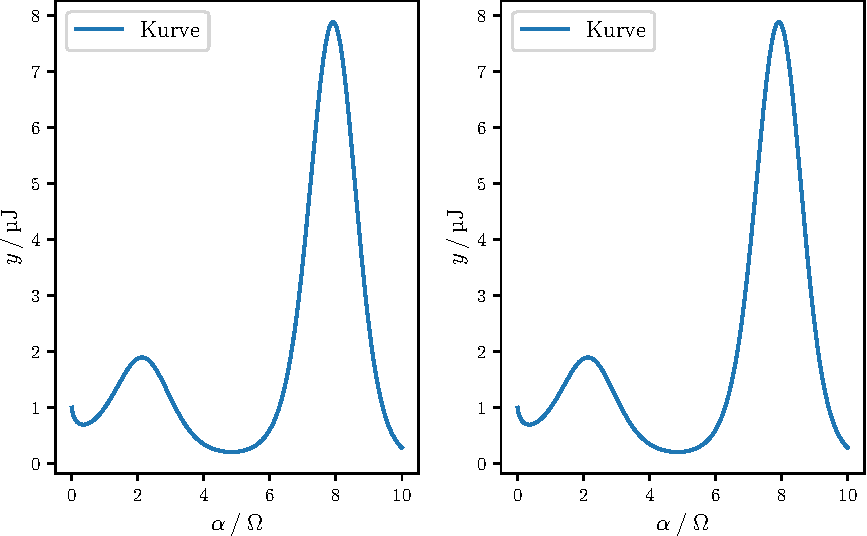
\includegraphics{plot.pdf}
  \caption{Kapazität gegen Anzahl an Extrema.}
  \label{fig:plot}
\end{figure}
\newpage
Das Verhältnis muss demnach annähernd linear mit der Kapazität ansteigen.
Die rechnerischen Werte für \(\nu_+\) ergeben sich aus:
\begin{equation}
  \omega^+ = \frac{1}{\sqrt{LC}} = 196.3832kHz
\end{equation}
bzw.
\begin{equation}
  \omega^+ = \frac{1}{\sqrt{L(C+C_{sp})}} = 192.0015kHz
\end{equation}
Um das theoretische Verhältnis zu ermitteln, werden die Theorie-Werte aus \autoref{tab:tab3} durch die errechneten Fundamentalfrequenzen von 192.0015kHz geteilt.
%Nicht die Schwebungsfrequenz...
%Nochmal Schwebungsfrequenz berechnen und Formeln hin.
Es folgen die Formeln für die Schwingungs- und die Schwebungsfrequenz sowie die Einhüllende:

\begin{equation}
 \nu =\frac{\omega^+ + \omega^-}{4\pi}
\end{equation}
\begin{equation} 
 \nu_{\symit{E}} = \frac{\omega^- - \omega^+}{4\pi}
\end{equation}
\begin{equation}
 \nu_{\symit{S}} = 2\nu_{\symit{E}}
\end{equation}

Daraus ergibt sich die Anzahl der Maxima:

\begin{equation}
 N_{\symit{max}} = \frac{\nu}{\nu_{\symit{S}}}
\end{equation}

\begin{table}
  \centering
  \caption{Hier sind die theoretische Schwingungsverhältnisse zu sehen.}
  \label{tab:tab6}
  \begin{tabular}{c c}
    \toprule
    \(C_K\) in nF & Verhältnis \(\frac{\omega^-}{\omega^+}\)\\
    \midrule
    2.03 & 1.338 \\
    3.00 & 1.239 \\
    4.00 & 1.184 \\
    5.02 & 1.149 \\
    6.47 & 1.117 \\
    8.00 & 1.096 \\
    9.99 & 1.077 \\
    \bottomrule
  \end{tabular}
\end{table}

\newpage

\begin{table}
  \centering
  \caption{Im Vergleich zu \autoref{tab:tab6} sind hier nun die  experimentelle Schwingungsverhältnisse, die mithilfe der oben genannten Methoden gemessen wurden, zu sehen.}
  \label{tab:tab7}
  \begin{tabular}{c c}
    \toprule
    \(C_K\) in nF & Verhältnis mit Maxima\\
    \midrule
    2.03 & 0.25 \\
    3.00 & 0.2 \\
    4.00 & 0.2 \\
    5.02 & 0.166 \\
    6.47 & 0.125 \\
    8.00 & 0.091 \\
    9.99 & 0.71 \\
    \bottomrule
  \end{tabular}
\end{table}

%Wissenschaftlicher Ausdruck? Abweichung der Messwerte ist noch nicht so groß.
%VERÄNDAERUNGGGGGGGGGGGGGGGGGGGGGGGGGGGGGGGGGGGGGGGGGGGGGGGGGGGGGGGGGGGGGGGGGGGGGGGGGGGGGGGGGGGGGGGGGGGGGGGGGGGGGGGGGGGGGGGGGGGGGGGGGGGGGGGGGGGGG
\newpage
\subsection{Lissajous-Figuren}

\begin{table}
  \centering
  \caption{Das sind die Fundamentalfrequenzen in Abhängigkeit zu den verschiedenen Kapazitäten des Kondensators \(C_K\) bei der Phasenverschiebung $\Delta\phi$= 0.}
  \label{tab:tab2}
  \begin{tabular}{c c c}
    \toprule
    \(C_K\) in nF & \(\nu_-\) in Hz & \(\nu_+\) in Hz\\
    \midrule
    1.01 & 47090 & 30450 \\
    2.03 & 39990 & 30440 \\
    3.00 & 37275 & 30440 \\
    4.00 & 35730 & 30440 \\
    5.02 & 34760 & 30440 \\
    6.47 & 33870 & 30440 \\
    8.00 & 33260 & 30440 \\
    9.99 & 32740 & 30440 \\
    \bottomrule
  \end{tabular}
\end{table}
%Alle Frequenzen, die gemessen wurden, keine Kreisfrequenzen
%"Fundamentalfrequenzen" ... okay'er Ausdruck? Yes.

\autoref{fig:plot2} und \autoref{tab:tab2} zeigen die Frequenzen, bei denen unter verschiedenen Kapazitäten die Phasenverschiebung 0 beträgt, also \(\omega^+\), oder \(\pi\), also \(\omega^-\).
Es ist sehr deutlich zu sehen, dass die Phasenverschiebung um \(\pi\) so gut wie immer bei der selben Frequenz erfolgt, unabhängig von der Kapazität.
\(\omega^-\) hingegen fällt mit zunehmender Kapazität ab.
\begin{figure}
  \centering
  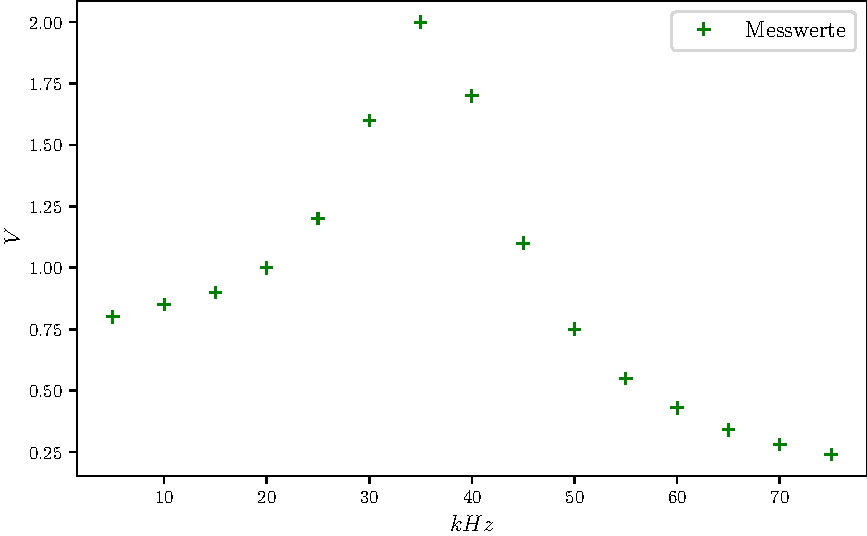
\includegraphics{plot2.pdf}
  \caption{Hier sind sowohl beide experimentell bestimmte Frequenzen, als auch die Theoriekurve von \(\nu_-\) und \(\nu_+\) im Verhältnis zu \(C_{\symit{k}}\) zu sehen. Es wird ersichtlich, dass keine große Diskrepanz zwischen den experimentell bestimmten Werten und den Berechnungen der Theorie besteht.}
  \label{fig:plot2}
\end{figure}
\newpage
Die Theorie-Werte für \(\nu_-\) weichen nur leicht ab:
\\
\begin{table}
  \centering
  \caption{Theoriewerte für \(\nu_-\)}
  \label{tab:tab3}
  \begin{tabular}{c c}
    \toprule
    C in nF & \(\nu_-\) in Hz\\
    \midrule
    1.01 & 49842.28\\
    2.03 & 41294.10\\
    3.00 & 38154.68\\
    4.00 & 36404.43\\
    5.02 & 35294.99\\
    6.47 & 34290.31\\
    8.00 & 33608.58\\
    9.99 & 33023.39\\
    \bottomrule
  \end{tabular}
\end{table}
Es wird beim Vergleich deutlich, dass die  Abweichungen von den gemessenen Werten sich mit zunehmender Kapazität \(C_k\) verkleinern. 
%angefangen bei 5.52\% bei 1.01nF bis hin zu nur 0.86\% bei 9.99nF.
%Wie ist Richard darauf gekommen??
\newpage
\subsection{Stromverlauf im gekoppeltem Schwingkreis}

\begin{table}
  \centering
  \caption{Hier sind die Spannungsamplituden bei steigender Frequenz zu sehen. Die Zeiten an denen diese Amplituden zu sehen sind, wurden auf der X-Achse des Oszillographen gemessen.}
  \label{tab:tab4}
  \begin{tabular}{c c c c c}
    \toprule
    \(C_K\) in [nF] & \(U_{2,1}\) [V] & \(U_{2,2}\) [V] & a in [ms] & b in [ms]\\
    \midrule
    2.03 & 1.75 & 1.4 & 17.5 & 29.5\\
    3.00 & 1.75 & 1.5 & 18 & 21.5\\
    4.00 & 1.75 & 1.55 & 18 & 16.5\\
    5.02 & 1.75 & 1.55 & 17.5 & 13.5\\
    6.47 & 1.75 & 1.6 & 17.5 & 10.5\\
    8.00 & 1.8 & 1.6 & 17.5 & 8.5\\
    9.99 & 1.8 & 1.6 & 18 & 6.5\\
    \bottomrule
  \end{tabular}
\end{table}
Die \autoref{fig:plot3} zeigt die Verteilung der Frequenzen \(\omega^\pm\) in Anhängigkeit der Kapazität von \(C_k\).
Wie auch schon bei \autoref{fig:plot2} zeigt \(\omega^-\) eine abfallende Kurve.
Um \(\omega^+\) und \(\omega^-\) zu erhalten, muss man die Parameter der Sweepfunktion miteinander verrechnen:
\begin{equation}
  \nu_+ = \frac{\nu_{\symit{end}}-\nu_{\symit{start}}}{0.16 \symit{s}}\cdot a + 25 \symup{kHz}
\end{equation}
und
\begin{equation}
  \nu_- = \frac{\nu_{\symit{end}}-\nu_{\symit{start}}}{0.16 \symit{s}}\cdot b + \nu_+
\end{equation}
Diese Rechnung wird bei allen Kapazitäten angewandt, die in \autoref{tab:tab5} zu sehen sind.\\
Somit ergebensich für die Werte:

\begin{table}
  \centering
  \caption{Hier sind die errechneten Frequenzwerte für \(\nu_+\) und \(\nu_-\) in Abhängigkeit von \(C_{\symit{K}}\).}
  \label{tab:tab5}
  \begin{tabular}{c c c}
    \toprule
    \(C_K\) in [nF] & \(\nu_+\) in [kHz] & \(\nu_-\) in [kHz]\\
    \midrule
    2.03 & 24.962 & 24.987\\
    3.00 & 24.972 & 24.928\\
    4.00 & 24.978 & 24.957\\
    5.02 & 24.978 & 24.965\\
    6.47 & 24.984 & 24.971\\
    8.00 & 24.978 & 24.967\\
    9.99 & 24.978 & 24.970\\
    \bottomrule
  \end{tabular}
\end{table}

\begin{figure}
  \centering
  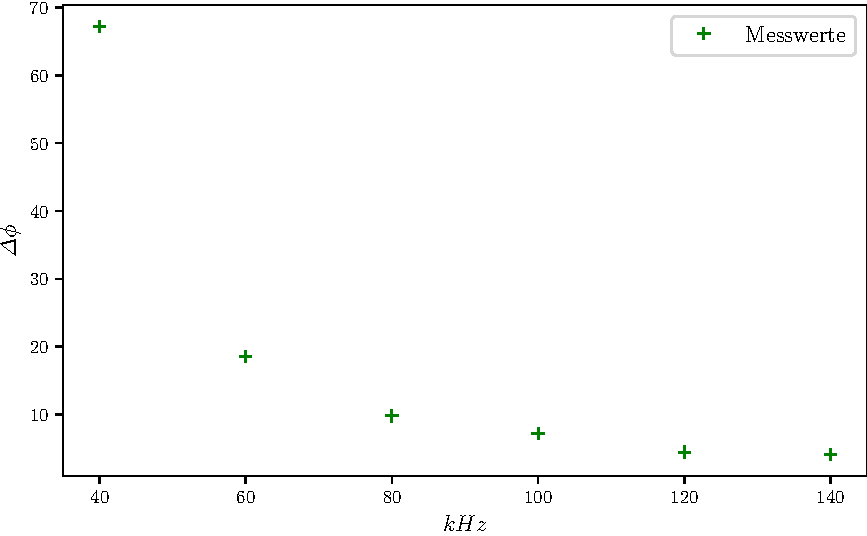
\includegraphics{plot3.pdf}
  \caption{Zu sehen ist hier das Verhältnis zwischen den Fundamentalfrequenzen und der Kapazität \(C_{\symit{k}}\).}
  \label{fig:plot3}
\end{figure}
Um den zugehörigen Strom zu bestimmen, verwendet man \autoref{eq:strom+} und \autoref{eq:strom-}:
\begin{equation}
  I_2 = |U| \cdot |L(\omega^\pm)| \quad\textrm{mit}\quad |U| = 8V
\end{equation}

In \autoref{tab:tabex} sind die Werte für $L(\omega^+)$ aufgetragen.

\begin{table}
  \centering
  \caption{Wird die \autoref{eq:strom+} zur Ermittlung des Wertes für \(L(\omega^+)\) verwendet, um dann daraufhin den theoretischen Wert von \(I_2\) zu ermitteln.}
  \label{tab:tabex}
  \begin{tabular}{c c c}
    \toprule
   \(C_{\symit{k}}\) [nF] & \(L(\omega^+)\) [A/V] $10^{-10}$ & \(I_2\) [A] \\
   \midrule
    1.01 & 20.626 & 165.00\\
    2.03 & 10.262 & 82.096\\
    3.00 & 6.944 & 55.552\\
    4.00 & 5.208 & 41.664\\
    5.02 & 4.150 & 33.200\\
    6.47 & 3.220 & 25.760\\
    8.00 & 2.604 & 20.832\\
    9.99 & 2.085 & 16.680\\
    \bottomrule
  \end{tabular}
\end{table}